\newcommand{\CLASSINPUTbaselinestretch}{1.3}
\documentclass[12pt, conference]{IEEEtran}
\usepackage{times}

% numbers option provides compact numerical references in the text. 
\usepackage[numbers]{natbib}
\usepackage{multicol}
\usepackage[bookmarks=true]{hyperref}
\usepackage{graphicx}
\usepackage{gensymb}
\usepackage{helvet}
\usepackage{tabulary}
\usepackage[clockwise]{rotating} % to rotate tables etc.
\usepackage{wrapfig}
\usepackage{ctable}
%\usepackage{booktable}
%\usepackage{cite}

\pdfinfo{
   /Author (Rohit Krishnan, Bunchhieng Soth)
   /Title  (Fisher Discriminant Analysis for Stroke Detection)
   /Subject (Robots)
   /Keywords (Robots;Overlords)
}

\begin{document}

\title{Fisher Discriminant Analysis for Stroke Detection}

\author{Rohit Krishnan, Bunchhieng Soth}

\maketitle

\begin{abstract}
The development of Medical assistive technology has become increasingly necessary in the last decade, fueled by the high cost and difficulty in finding trusted in-home nursing services. More recently, growth in robotic technology has been expedited by intelligent computer vision, latest battery technology, and energy efficient parts. However, little has been done to bridge robotics, Computer Vision (CV), and medical assistance in a consumer-grade and economical manner. In this paper, we propose an affordable indoor Unmanned Aerial Vehicle (referred to as a Baymax) equipped with an Intel RealSense depth sensing camera to detect an incurring stroke on a patient. In particular, this study highlights the computer vision tasks involved in identifying a Facial Palsy from the images supplied by the camera. Our use of Fisher Discriminant Analysis for the classification of Facial Palsy will also be compared in performance to other methods of classification –such as Support Vector Machine.
\end{abstract}

\IEEEpeerreviewmaketitle

\begin{figure}
\begin{center}
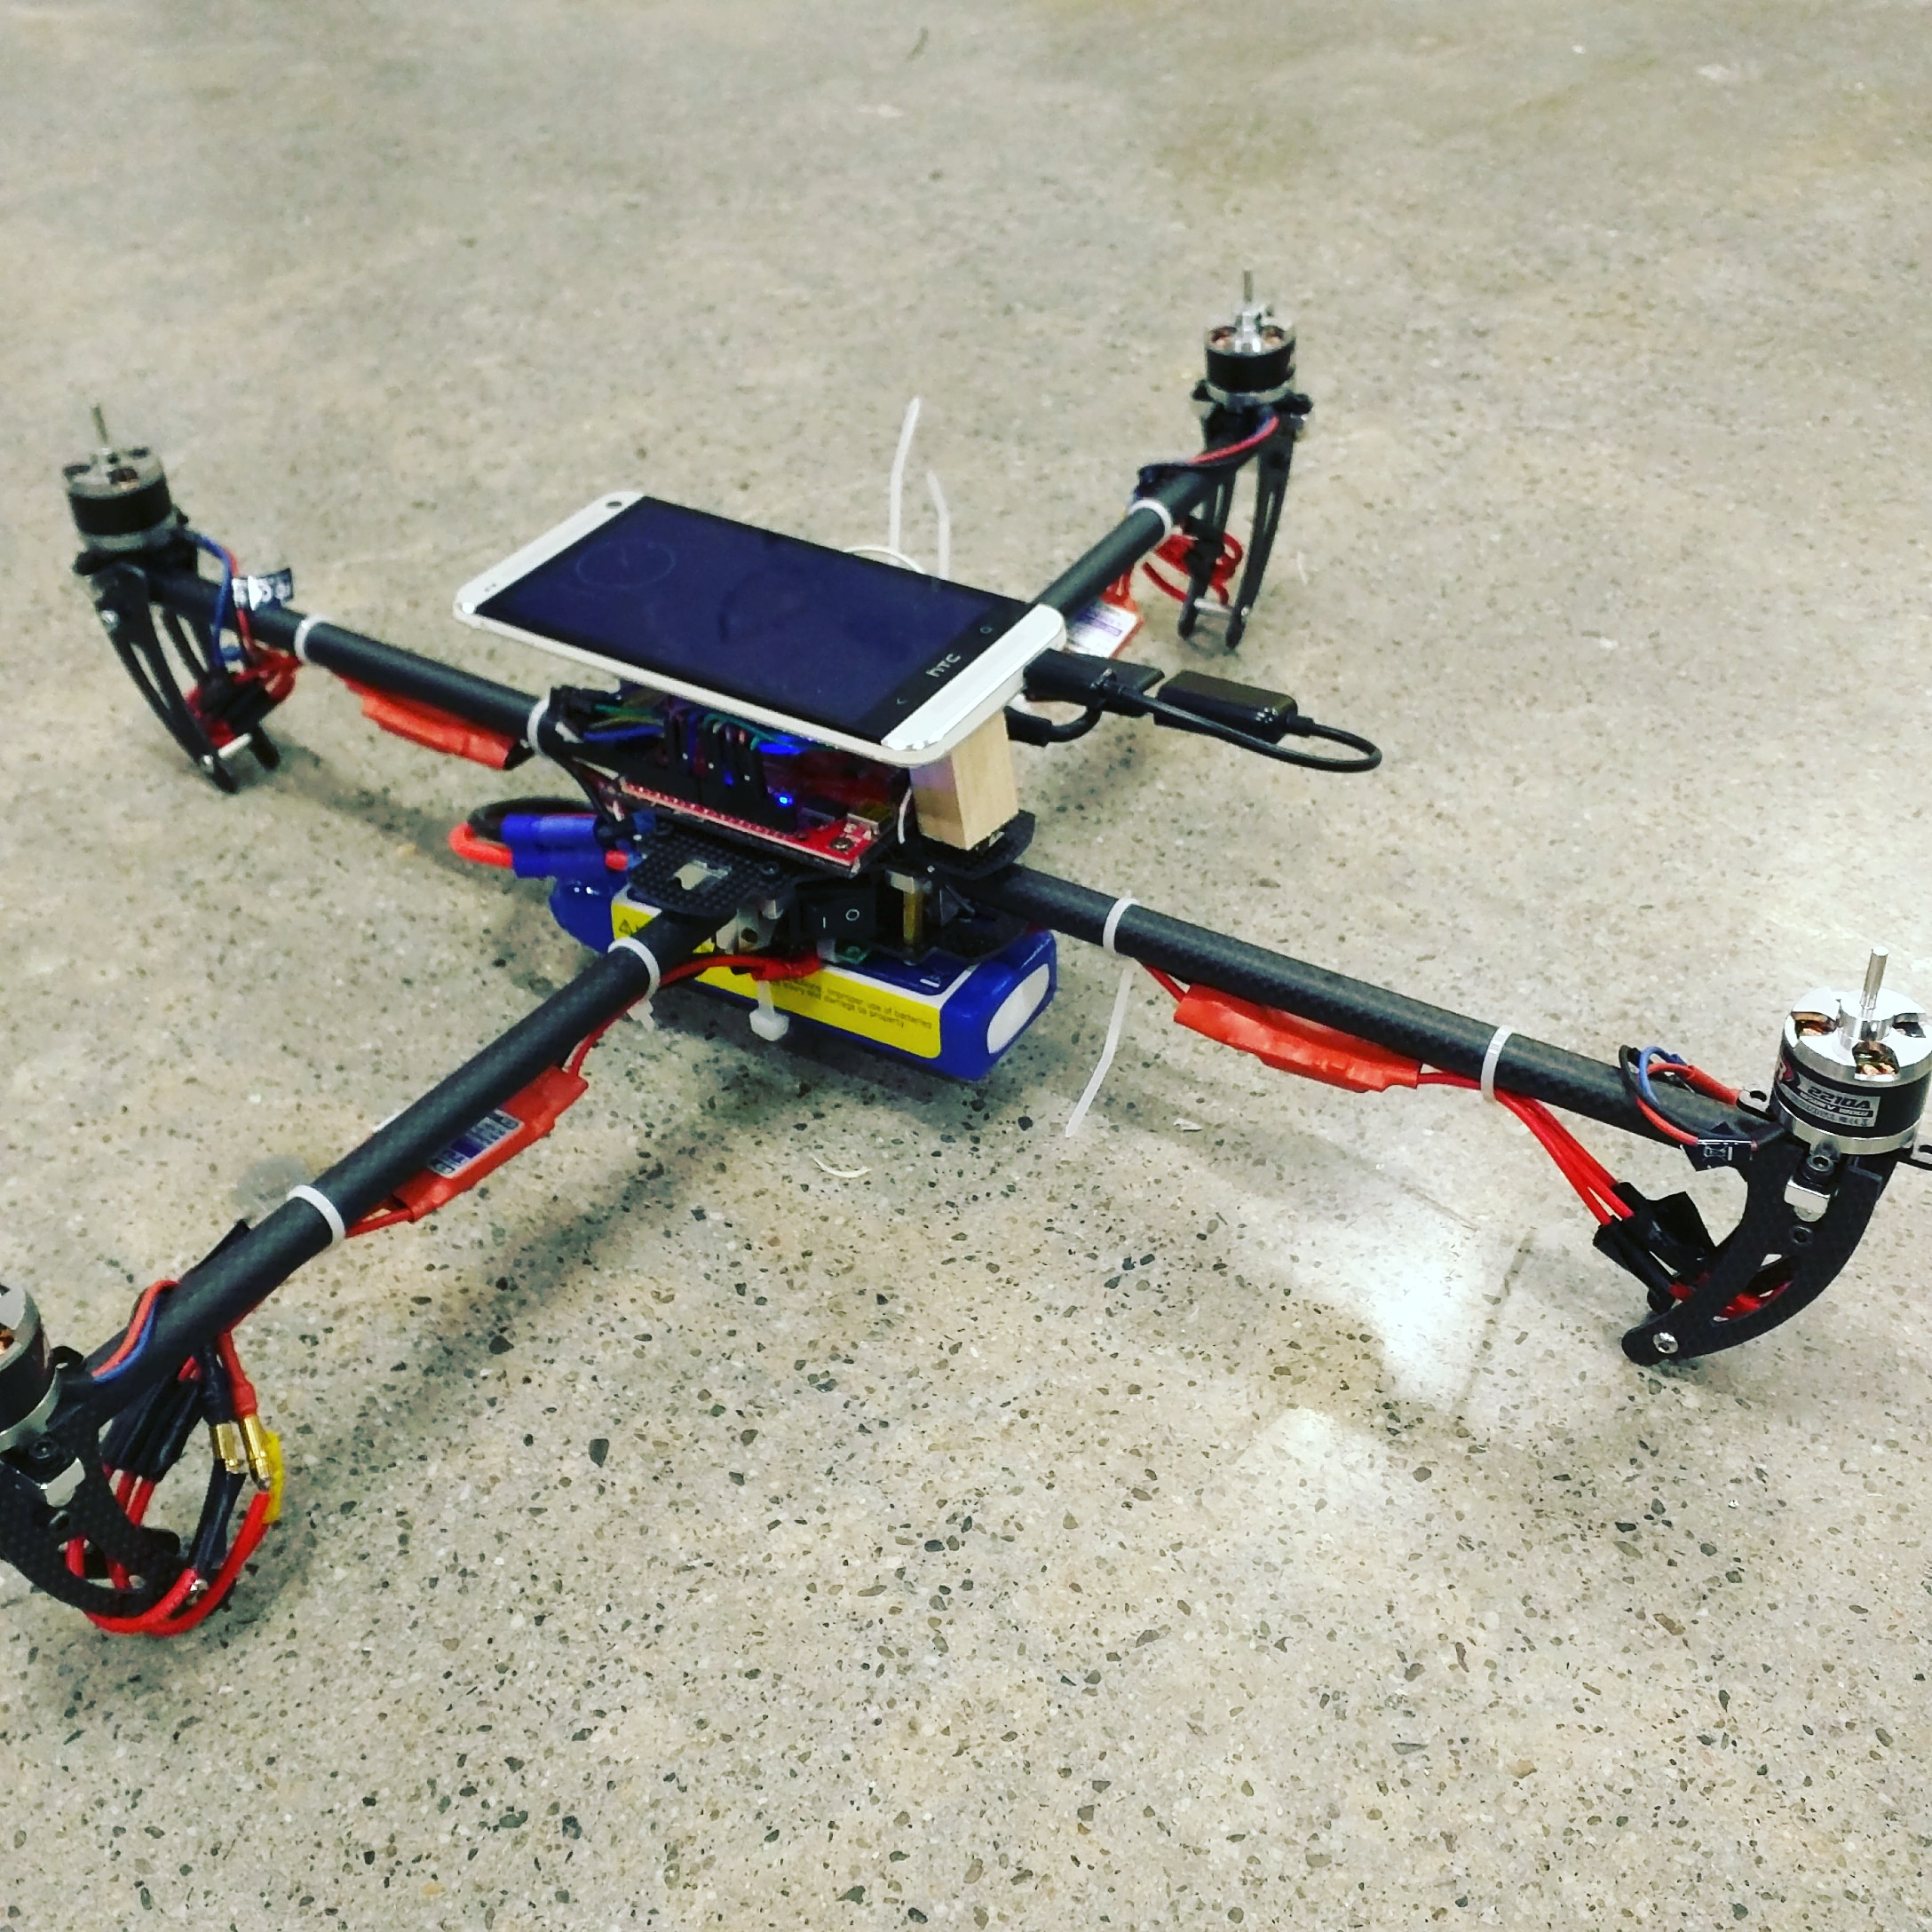
\includegraphics[width=7.6cm]{pictures/dronepic}
\end{center}
\caption{Autonomous quadcopter which uses Computer Vision to identify strokes. Camera and propellers have been detached.}
\label{dronepic}
\end{figure}

\section{Introduction}
The two primary issues Baymax will attempt to mitigate are the cost of home health care nurses, and the safety hazards of family members acting as an informal substitute for Registered Nurses. The Centers for Medicare \& Medicaid Services (CMS) estimates over 10,800 home health agencies providing care for over 3.4 million elderly or disabled patients \cite{7}. Unfortunately, the eligibility for Home Health Benefit from Medicare is only limited to patients requiring part-time or non-continuous patient care for fewer than 21 contiguous days\cite{8}. To those who are not covered by the Medicare program, the approximate cost of a home health aide is 21 per hour without extra charges for additional services \cite{9}; this leaves the option for full-time nurses unaffordable for those needing intermittent care. One of the more affordable alternatives to having an in-home nurse is the use of an Assisted Living Facility, which provides a one-bedroom unit for approximately \$3,000 per month \cite{9}. However, the Centers for Disease Control and Prevention (CDC) estimates 66\% of people hospitalized for stroke are over the age of 65 years \cite{10}, and the American Association of Retired People (AARP) reports the vast majority of Americans (89\%) of ages 50+ want to remain in their own homes as long as they can \cite{6}, which leaves an Assisted Living Facility inconvenient for the majority of stroke victims. The latter issue, and the more common alternative to Medicare and Assisted Living Facilities, is the use of family members and untrained caregivers helping their loved ones at home. Although there are over 34 million family care-givers in the United States \cite{6} who practice this, there is a lack of oversight, prompt response, and experience that would otherwise be offered by a formal Registered Nurse \cite{11}. Our solution, Baymax, is an assistive drone that will aid recovering stroke victims who require frequent monitoring for facial palsy. Although our solution is novel to home health care and medical assistance, there are a number of non-trivial computational challenges outlined in this paper.

\section{Mechanical Apparatus}
Although the intrinsic of the electrical and mechanical components of the quadcopter will not be discussed within this paper, it is important to understand the nature of the images that are taken from the quadcopter and the apparatus that we use to gather this data. As shown in Fig 1, the quadcopter consists of a carbon fiber frame with an Android phone connected via a USB OTG cable to an Intel RealSense 3D depth-sensing camera. The Android phone then uses the linux libUVC framework to receive the image in YUV format and perform the necessary processing described in the later portions to classify the object as a normal face or one with palsy. The drone is capable of flying to eye-level height and taking a picture of the patient’s face.

\break

\section{Machine Learning Overview}
The binary classification of human faces is not a relatively new problem, and has been approached in a variety of methods to solve a number of different issues, including the classification of gender among a set of images. However, there are a number of optimizations which could be learned from research in face classification to be applied towards classifying stroke victims. Namely, this project focuses on the use of Gabor filters and Fisher Discriminant Analysis –as proposed by a number of other works (such as \cite{1}) towards the classification of Bell’s Palsy. 

\subsection{The Basics}
The high level description of the problem involved is to classify an image that is captured from the camera and determine the probability that the image captured includes a face that is experiencing Bell's Palsy - A muscle weakness on one side of the face that is indicative of a stroke. To do this, the practice of "supervised" Machine Learning involves sifting through hundreds of images of individuals' faces which are marked as positive or negative for experiencing Bell's facial palsy, and identifying "features" which are representative of the proper classification. Once the machine has "learned" the best possible decision boundary to classify an image, it will "validate" what it has learned and improve on its parameters by testing against a cross-validation set. Finally, when it has finished optimizing the parameters to maximize fit the CV set while minimizing overfitting the data, it will test this against the test set. This set will determine the overall accuracy, precision, recall, and F-Score of the algorithm. 

\subsection{Linear Discriminant Analysis} \label{sec:Basics}
Due to the high dimensionality of the image being supplied, one of steps applied to resolve this is Linear Discriminant Analysis - a tool used for dimensionality reduction. Ronald A. Fisher, in 1936, described Linear Discriminant Analysis in "The Use of Multiple Measurements in Taxonomic Problem"\cite{2}, but it has since been used as a pre-processing method to the binary classification task as described in this project. The intention of this procedure is to bring the high-demensional image to a lower dimension and prevent overfitting among the hundreds of images we will be training with. In this specific instance, we will project the 2500 dimensional (50px*50px) image into a lower feature space to preserve the information necessary in classifying the image while reducing the amount of information sent to training. This will also reduce the time it takes to compute the training model. 


\subsection{Principal Component Analysis} \label{sec:Basics}
Similar to Linear Discriminant Analysis, PCA is also a tool used for lowering the dimensionality of an image by linearly transforming the image. However, PCA is indiscriminant to the class label of the image and will not be dependend on whether the image contains a regular face or palsy. Instead, it is used as a feature extraction tool; PCA is an unsupervised learning method that is most useful when the class labels are unknown. In this proposal, we will be using PCA and LDA in conjunction for dimensionality reduction, feature extraction, and minimizing overfitting. This method, also known as Fisher Discriminant Analysis, is used for a number of applications, including face recognition as in \cite{2}.

\break

\subsection{Fisher Discriminant Analysis} \label{sec:Basics}
Fisher Discriminant Analysis exploits the findings of both the above methods by minimizing the within-class variance, and maximizing the between-class variance, by proposing the following optimization problem:
\begin{equation}\label{equ:fisher}
J(w) = \frac{w^TS_Bw}{w^TS_Ww}
\end{equation}
where $w$ is the optimal weight vector to be calculated, $S_B$ is the between-classes scatted matrix, and $S_W$ is the within-classes scatter matrix. The cost function J(w) tries to minimize the within-classes scatter matrix and maximize the between-classes scatter matrix. Due to the scatter matrices being proportional to the covariance matrices, J is redefined using the covariance matrices. The two variables $S_B$ and $S_W$ can each be calculated separately for the optimal solution using the following:

\begin{equation}
	S_B = \sum_{i=1}^{c} N_i*(\mu_i - \mu)*(\mu_i - \mu)^T	
\end{equation}


$\mu$ and $\mu_i$ are the total mean and mean of class i of the matrix X projected into the N-C dimensional subspace by applying Principal Component Analysis. This matrix, X - the training matrix, and the construction of it, will be discuss later in \ref{sec:Basics}.

\begin{equation}
	S_W = \sum_{i=1}^{c} \sum_{x_k \in X_i} (x_k - \mu_i) * (x_k - \mu_i)^T
\end{equation}

$X_i$ are the samples from matrix X (training vector) that are of class i, and $x_k$ is a sample of $X_i$.


\section{Implementation details} \label{sec:Basics}
Without further detail on the Fisher Discriminant Analysis itself, the rest of this paper will focus on the methods required to feed the set of processed images we have to the Fisher LDA algorithm that is offered by the OpenCV (Open Computer Vision) framework.  

\subsection{Training Matrix}
The OpenCV Fisher LDA algorithm requires that our training set be a single matrix. To achieve this, we take each image (represented as 50px by 50px matrix) and map it such that each row of our training matrix X will consist of all the bytes in a single image. For our training set of 1100 images each at 50px by 50px, we result in a training matrix of 1100x2500. Running the Fisher algorithm on this matrix will result in the eigenvectors and eigenvalues corresponding to our cost function $J(w)$. We can then take a given image to classify and project it against the given eigenvector and use nearest-neighbor matching to determine the class that best fits the image.

\begin{figure}
\begin{center}
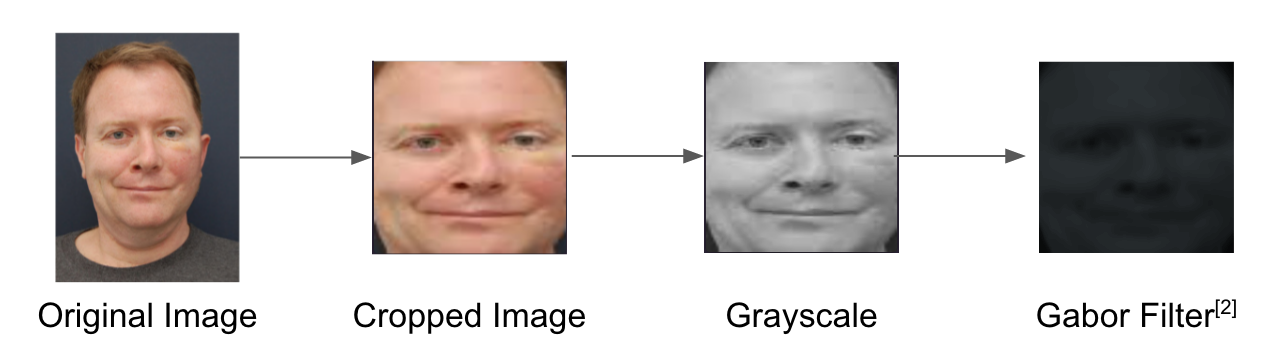
\includegraphics[width=8.6cm]{pictures/imageproc}
\end{center}
\caption{Various stages illustrated of the pre-processing algorithm.}
\label{imageproc}
\end{figure}

\section{Image Pre-Processing} 
Arguably, the most important part of any image classification task is pre-processing the image. In this particular implementation, the following pre-processing tasks were applied:
\begin{flushleft}
\begin{enumerate}
	\item Download raw image
	\item Crop image to 200x200 size
	\item Convert to grayscale
	\item Apply Gaussian kernel convolution
	\item Apply Gabor kernel convolution
\end{enumerate}	
\end{flushleft}
The first step in pre-processing involves further reducing the dimensionality by cropping the image to a rectangle around just the Face by using three HAAR classifiers to detect Face, Mouth, and an Eye. We only search the image for a single eye due to the palsy causing difficulty in detecting the other eye. Next, we convert the image to grayscale (single channel with intensities) due to color not being correlated to the classification of facial palsy, and due to the large variance caused by lighting. After this, a Gaussian blur filter is applied on the image to reduce the amount of noise that is within the image. Finally, we apply a Gabor kernel convolution on the image as suggested by Zhang\cite{4}. The Gabor kernel is also justified by its similar modeling of our visual cortex's detection of edges, which was first discovered by Marĉelja in 1980\cite{3}. 
\section{Evaluation} 
\begin{table*}
\begin{center}
\caption{Comparison of Baymax's Fisher Discriminant Analysis against Song\cite{1} et al's Support Vector Machine} % title of Table
\centering % used for centering table
\begin{tabular}{p{4.8cm} p{2cm}  p{2.3cm}  p{2cm}  p{2.4cm} } % centered columns (4 columns)
\hline\hline %inserts double horizontal lines
Set & Palsy Images & Regular Images & F-Measure & Recall \\ [0.5ex]
%heading
\hline % inserts single horizontal line
FLDA & 55 & 189 & 85.2\% & 94.55\% \\ % inserting body of the table
SVM & 46 & 21 & 95.42\% & 97.14\% \\ % inserting body of the table
[1ex] % [1ex] adds vertical space
\hline %inserts single line
\end{tabular}
\label{table:metrics} % is used to refer this table in the text
\end{center}	
\end{table*}

Table \ref{table:metrics} above compares our implementation of the Fisher LDA algorithm against the Support Vector Machine developed by Song el Al\cite{1} to profile the grade of Facial Palsy displayed by patients. The following subsections will highlight the procedure in optimizing the parameters and measuring against the test set to calculate the F-Measure and Recall.

\subsection{Measuring Performance}
In order to measure the performance of any tuning that is made to the parameters or the learning algorithm, a balanced measurement needs to be calculated. In statistical analysis, the F-score is used as a method to measure the algorithm's accuracy, by weighting the harmonic mean of the precision and recall.

\begin{equation}
	P = 100 * \frac{TruePositive}{TruePositive + FalsePositive}
\end{equation}
\begin{equation}
	R = 100 * \frac{(TruePositive}{TruePositive + FalseNegative}
\end{equation}
\begin{equation}
	F_1 = 2 * \frac{P * R}{P + R}
	\label{eq:fscore}
\end{equation}

Equation \ref{eq:fscore} will be used in the validation of our algorithm against the cross-validation set, the test set, and other methods (such as SVM proposed by \cite{1}).

\subsection{Optimizing with Cross-Validation set}
Prior to optimizing the Gabor filter parameters using the CV set, we first try an initial set of random parameters to measure the accuracy/precision before and after optimizing.

\begin{itemize}
	\item $\sigma=0.5$ - Std. deviation of gaussian envelope
	\item $\gamma=0.5$ - Spatial aspect ratio for Gabor filter.
	\item $\theta=0$ - Orientation of the normal to the Gabor function.
\end{itemize}

With these parameters, the initial test resulted in the above accuracy/precision (the calculation for which is described in the prior subsection).

Upon final optimization, the following metrics are used to calculate the F-score:
\begin{itemize}
	\item True-Pos: 52
	\item True-Neg: 186
	\item False-Pos: 15
	\item False-Neg: 3
	\item Precision: 77.6119\%
	\item Recall: 94.5455\%
	\item F1-Score: 85.2459\%
\end{itemize}



\begin{table}
\begin{center}
\caption{Baymax Fisher LDA before optimization} % title of Table
\centering % used for centering table
\begin{tabular}{c c c c c } % centered columns (4 columns)
\hline\hline %inserts double horizontal lines
Set & Palsy Images & Regular Images & F-Measure & Recall \\ [0.5ex]
%heading
\hline % inserts single horizontal line
FLDA & 55 & 189 & 57.8\% & 40.57\% \\ % inserting body of the table
[1ex] % [1ex] adds vertical space
\hline %inserts single line
\end{tabular}
\label{table:metrics} % is used to refer this table in the text
\end{center}	
\end{table}

Although the performance of these parameters are worse than random probability, visual analysis of the image produced after applying the Gabor Filter with the parameters above shows a black image with edges that do not focus on the mouth or the eyes (which are the critical portions of the face for detecting Palsy). To improve this, we add another layer to the training phase which runs through a number of different values for $\sigma$, $\gamma$, and $\theta$, to determine which results in the greatest F-Score against the cross-validation set. Finally, this value is used in measuring against the test.


After running through the iterative process, the best values for the parameters were the following:
\begin{itemize}
	\item $\sigma=1.2$
	\item $\gamma=1.2$
	\item $\theta=1.37445$
\end{itemize}


\begin{table}
\begin{center}
\caption{Baymax Fisher LDA after optimization} % title of Table
\centering % used for centering table
\begin{tabular}{c c c c c } % centered columns (4 columns)
\hline\hline %inserts double horizontal lines
Set & Palsy Images & Regular Images & F-Measure & Recall \\ [0.5ex]
%heading
\hline % inserts single horizontal line
FLDA & 52 & 186 & 85.2\% & 94.55\% \\ % inserting body of the table
[1ex] % [1ex] adds vertical space
\hline %inserts single line
\end{tabular}
\label{table:metrics} % is used to refer this table in the text
\end{center}	
\end{table}


\break

\section{Conclusion and future work} 
Although the use of Linear Discriminant Analysis for the binary classification of individuals with Facial Palsy does not allow polynomial decision boundary for complex pattern recognition as in other networks such as SVM\cite{1}, we were able to demonstrate a very close level of accuracy and ability of detection simply by tuning the parameters of the Gabor Filters to better fit the cross-validation set, and aggregating more images. 
There are a number of optimization which can be made to our current methods. Firstly, rather than the use of the public domain (Google Images) for aggregation and hand-selection of the Facial Palsy images, a better dataset would be attained from a local Hospital or a neurology department with the consent of patients. Next, it would be prudent to test the use of the pre-processing techniques (such as application of Gabor Filter convolution) illustrated earlier against a Support Vector Machine to potentially increase the accuracy and develop polynomial decision boundaries.  

\break
\section{Roles and Responsibilities}
The majority of this assignment has been performed in the presence of both members, however there are certain portions which were completed individually which are defined below:

\begin{itemize}
	\item \textbf{Downloading Images} - Approximately 10k images were downloaded in bulk using a software written in GoLang by Bunchhieng.
	\item \textbf{Initial FLDA test} - Initial test program using OpenCV to read an image and pass it to Fisher LDA written by Rohit.
	\item \textbf{Initial SVM test} - Some amount of minor testing was done with applying SVM to this project by Bunchhieng, but due to time constraints was not ready for data analysis and comparison. 
\end{itemize}


%% Use plainnat to work nicely with natbib. 
\cleardoublepage
\centering
\center
\bibliographystyle{IEEEtran}
%$\bibliographystyle{plainnat}
\bibliography{bibliography/bibliographyRSS.bib}
\end{document}


